
\let\negmedspace\undefined
\let\negthickspace\undefined
\documentclass[journal]{IEEEtran}
\usepackage[a5paper, margin=10mm, onecolumn]{geometry}
%\usepackage{lmodern} % Ensure lmodern is loaded for pdflatex
\usepackage{tfrupee} % Include tfrupee package

\setlength{\headheight}{1cm} % Set the height of the header box
\setlength{\headsep}{0mm}     % Set the distance between the header box and the top of the text

\usepackage{gvv-book}
\usepackage{gvv}
\usepackage{cite}
\usepackage{amsmath,amssymb,amsfonts,amsthm}
\usepackage{amsmath}
\usepackage{algorithmic}
\usepackage{graphicx}
\usepackage{textcomp}
\usepackage{xcolor}
\usepackage{txfonts}
\usepackage{listings}
\usepackage{enumitem}
\usepackage{mathtools}
\usepackage{gensymb}
\usepackage{comment}
\usepackage[breaklinks=true]{hyperref}
\usepackage{tkz-euclide} 
\usepackage{listings}
% \usepackage{gvv}                                        
\def\inputGnumericTable{}                                 
\usepackage[latin1]{inputenc}                                
\usepackage{color}                                            
\usepackage{array}                                            
\usepackage{longtable}                                       
\usepackage{calc}                                             
\usepackage{multirow}                                         
\usepackage{hhline}                                           
\usepackage{ifthen}                                           
\usepackage{lscape}
\usepackage{circuitikz}
\tikzstyle{block} = [rectangle, draw, fill=blue!20, 
    text width=4em, text centered, rounded corners, minimum height=3em]
\tikzstyle{sum} = [draw, fill=blue!10, circle, minimum size=1cm, node distance=1.5cm]
\tikzstyle{input} = [coordinate]
\tikzstyle{output} = [coordinate]


\begin{document}

\bibliographystyle{IEEEtran}
\vspace{3cm}

\title{4.8.14}
\author{AI25BTECH11018-Hemanth Reddy}
 \maketitle
% \newpage
% \bigskip
{\let\newpage\relax\maketitle}

\renewcommand{\thefigure}{\theenumi}
\renewcommand{\thetable}{\theenumi}
\setlength{\intextsep}{10pt} % Space between text and floats


\numberwithin{equation}{enumi}
\numberwithin{figure}{enumi}
\renewcommand{\thetable}{\theenumi}

\textbf{Question:}\\

Find the position vector of the foot of perpendicular and the perpendicular distance from the point  $ \vec{P}$ with position vector $  2\hat{i}  + 3  \hat{j}  + \hat{k} $ to the plane \textbf{r} $\cdot$ ( $ 2\hat{i}  +   \hat{j}  + 3\hat{k}$) -26 = 0.
 Also find image of $ \vec{P}$  in the plane.\\
\textbf{Solution:}\\
\begin{align}
   \text{ The position vector of point }  \vec{P} \text{ is }
  \textbf{p} = \myvec{ 2 \\ 3 \\ 1 } 
\end{align}
 The normal vector of the plane is 
\begin{align}
    \textbf{n} = \myvec{ 2 \\ 1 \\ 3 }
\end{align}



The plane equation is
\begin{align}
    \textbf{p}^T \cdot \textbf{n} - 26 = 0
\end{align} \\

1. Perpendicular Distance\\

The dot product $\textbf{p} \cdot \textbf{n}$ is given by the matrix multiplication $\textbf{p}^T \textbf{n}$.\\

\begin{align}
    \textbf{p}^{T} \textbf{n} = \myvec{ 2 & 3 & 1 } \myvec{ 2 \\ 1 \\ 3 } = (2)(2) + (3)(1) + (1)(3) = 10
\end{align}
 

\begin{align}
    |\textbf{n}| = \sqrt{\textbf{n}^T \textbf{n}} = \sqrt{\myvec{ 2 & 1 & 3 } \myvec{ 2 \\ 1 \\ 3 }} = \sqrt{4+1+9} = \sqrt{14}
\end{align}





The perpendicular distance d is:
\begin{align}
    d = \frac{|\textbf{p}^T \textbf{n} - 26|}{|\textbf{n}|} = \frac{|10-26|}{\sqrt{14}} = \frac{16}{\sqrt{14}}
\end{align}


2. Foot of Perpendicular\\

The position vector of the foot of the perpendicular    $\textbf{q}$ is:

\begin{align}
    \textbf{q} = \textbf{p} - \frac{(\textbf{p}^T \textbf{n} - 26)}{|\textbf{n}|^2} \textbf{n}
\end{align}
\begin{align}
  \textbf{q}  = \myvec{ 2 \\ 3 \\ 1 } - \frac{10 - 26}{14} \myvec{ 2 \\ 1 \\ 3 } = \myvec{ 2 \\ 3 \\ 1 } + \frac{16}{14} \myvec{ 2 \\ 1 \\ 3 }
\end{align}


\begin{align}
    \textbf{q} = \myvec{ 2 \\ 3 \\ 1 } + \frac{8}{7} \myvec{ 2 \\ 1 \\ 3 } = \myvec{ 2 + 16/7 \\ 3 + 8/7 \\ 1 + 24/7 } = \myvec{ 30/7 \\ 29/7 \\ 31/7 }
\end{align}


So the position vector of the foot of the perpendicular is $\frac{30}{7}\hat{i} + \frac{29}{7}\hat{j} + \frac{31}{7}\hat{k}$.

3. Image of $ \vec{P}$\\

The position vector of the image $\textbf{P'}$, is:\\

\begin{align}
     \textbf{P'} = 2\textbf{q} - \textbf{P} = 2 \myvec{ 30/7 \\ 29/7 \\ 31/7 } - \myvec{ 2 \\ 3 \\ 1 } = \myvec{ 60/7 - 14/7 \\ 58/7 - 21/7 \\ 62/7 - 7/7 } = \myvec{ 46/7 \\ 37/7 \\ 55/7 }
\end{align}

So the position vector of the image is $\frac{46}{7}\hat{i} + \frac{37}{7}\hat{j} + \frac{55}{7}\hat{k}$.

\begin{figure}
    \centering
    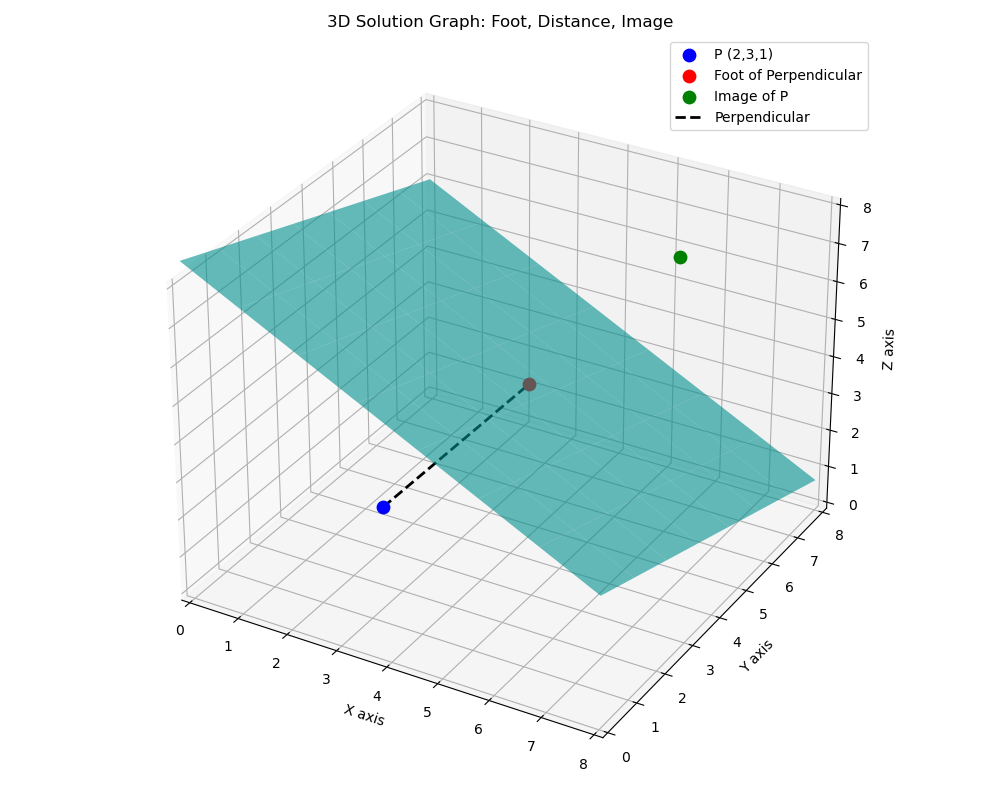
\includegraphics[width=1\linewidth]{figs/3d_plane_solution.png}
    \caption{}
    \label{fig:placeholder}
\end{figure}

\end{document}
